\section{What are Polyrhythm and Cross-rhythm?}

In the \textit{New Music Dictionary} (40th edition, 1996) published by Ongaku no Tomo Sha, "polyrhythm" is defined as "\textbf{a phenomenon in which contrasting rhythms are used simultaneously in two or more voices, also called cross-rhythm}"\cite{asaka:01}. The dictionary also cites the opening of J.S. Bach's "Sinfonia No. 9" as an example, noting that "\textbf{it is generally distinguished from the rhythmic symmetry that promotes the independence of voices inherent to polyphony}"\cite{asaka:01}. However, this suggests that even today, the definition of "polyrhythm/cross-rhythm" has not been established in a definitive manner. Furthermore, Yoda and Ono point out in their \textit{Music Theoretical Analysis of Polyrhythm Typology} that "\textbf{even by consulting only three music dictionaries, it becomes clear that the definition of polyrhythm is extremely diverse and ambiguous. Rhythm research has been historically neglected compared to harmony and other elements}"\cite{yoda-ono:01}, and they attempt to present a typology of polyrhythms. The fact that rhythm research has not been given as much weight as harmony can also be understood from Jean-Yves Bosseur's \textit{88 Keywords to Understanding Contemporary Music}, where most of the techniques discussed concern phonology, temperament, and acoustics, even in contemporary music. However, while the typology conducted by Yoda and Ono provides detailed analysis, it is classified using Western musical terminology that is not common in contemporary popular music. Here, separately from Yoda and Ono's analysis, we will examine "polyrhythm/cross-rhythm" in light of contemporary "popular music" situations, referring to "African polyrhythm" as the foundation for definition, and addressing "polyrhythm/cross-rhythm" as something that "Western music" has overlooked and as the present state of "popular music."

In this paper, we will explain the definition of polyrhythm based on African rhythms as "non-Western music," establish our definition of "polyrhythm/cross-rhythm," and then examine the "polyrhythmic/cross-rhythmic" nature of rhythms from Indian, Middle Eastern, and Latin genres. Subsequently, we will similarly examine "Western music" and "popular music," and finally consider the current state of "Western music" and "popular music" with regard to rhythm.

\subsection{Polyrhythm/Cross-rhythm in Non-Western Music}
\subsubsection{Africa}

Kikuchi and Otani state that "\textbf{one cycle of 12 is the prototype of polyrhythm in African music}"\cite{kikuchi-ootani:01} and that "\textbf{the basic polyrhythm of Africa is a cross between 4-beat and 3-beat time}"\cite{kikuchi-ootani:01}. This tendency can be affirmed from Tsukada's discussion of Brandel's vertical hemiola in \textit{The Truth About African Music} and from "the relationship between rhythm patterns (standard rhythm patterns) and beats coexisting in Africa"\cite{tsukada:01}.

Regarding Brandel's vertical hemiola, Tsukada states the following: "\textbf{Let us focus on the relationship between the song and hand claps in 'Song at Sunset' (Figure \ref{fig:figure_14}). The hand claps consistently proceed in 6/8 time, that is, in 2-division, so in the sections where the melody proceeds in 3/4 time (measures 1, 2, 5, and 7), rhythm patterns of 2-division and 3-division are simultaneously combined}"\cite{tsukada:01}. This is what Brandel calls vertical hemiola. Tsukada also describes this vertical hemiola as "\textbf{the most primitive form of African polyrhythm}"\cite{tsukada:01}. Furthermore, he states that "\textbf{if we consider that the complex polyrhythms of Africa are a highly developed form of this prototypical rhythm structure, then this vertical hemiola is precisely the characteristic African rhythm structure that Jones repeatedly emphasized in his polyrhythm theory, and the hand clap rhythm seen in 'Song at Sunset' is what Agawu calls 'the 6/8 time consistently present in the background of the piece'}"\cite{tsukada:01}, thus relating it to past polyrhythm research and demonstrating its validity.

\begin{figure}[ht]
\centerline{
	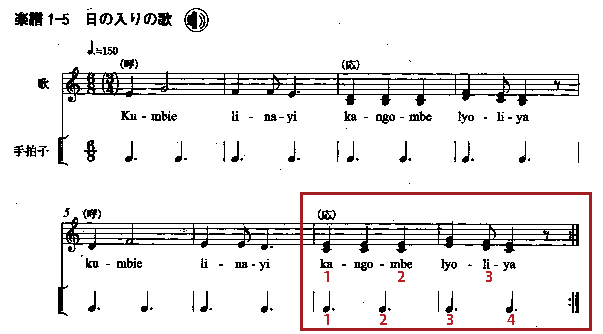
\includegraphics[
 width=\textwidth]{./PDF/figure_14.pdf}
}
\caption{Kenichi Tsukada (\textit{The Truth About African Music} p.41, Score 1-5, 2016)\\
In measures 1, 3, 5, and 7, the form of Brandel's vertical hemiola with 2-beat and 3-beat can be observed. Red frames and red text added by the author. The structure where "3-beat and 4-beat cross," as described by Kikuchi and Otani, can be seen.}
\label{fig:figure_14}
\end{figure}

The "prototype of African music polyrhythm" presented by Kikuchi and Otani can also be observed in Figure \ref{fig:figure_14} cited in Tsukada's discussion of vertical hemiola. Focusing on measures 7 and 8 enclosed in the red frame in Figure \ref{fig:figure_14}, and viewing these two measures as one unit of 12 beats, we can see that the hand claps are struck evenly four times. Furthermore, focusing on the quarter notes on beats 1 and 3 of measure 7 in the song, and the eighth note on beat 2 of measure 8, we can identify three evenly spaced strike points within the whole, confirming the same form with a 12-beat cycle: the song at 4+4+4, and the hand claps at 3+3+3+3 in eighth notes.

Regarding the 12-beat cycle rhythm pattern, "\textbf{as soon as one crosses the Sahara Desert from the north of the African continent, this rhythm pattern can suddenly be heard everywhere}"\cite{tsukada:01}, and its basic rhythm is summarized as shown in Figure \ref{fig:figure_15}. Furthermore, as shown in Figure \ref{fig:figure_16}, this basic rhythm is such that "\textbf{when Africans perform the standard rhythm pattern, they perform while feeling the eighth note as the 'basic pulse'}"\cite{tsukada:01}, and moreover, "\textbf{when performing the standard rhythm pattern, they feel three of these basic pulses as one unit (beat)}"\cite{tsukada:01}. From this, it can be considered that performances have been conducted in the form defined by Kikuchi and Otani.

\begin{figure}[ht]
\centerline{
	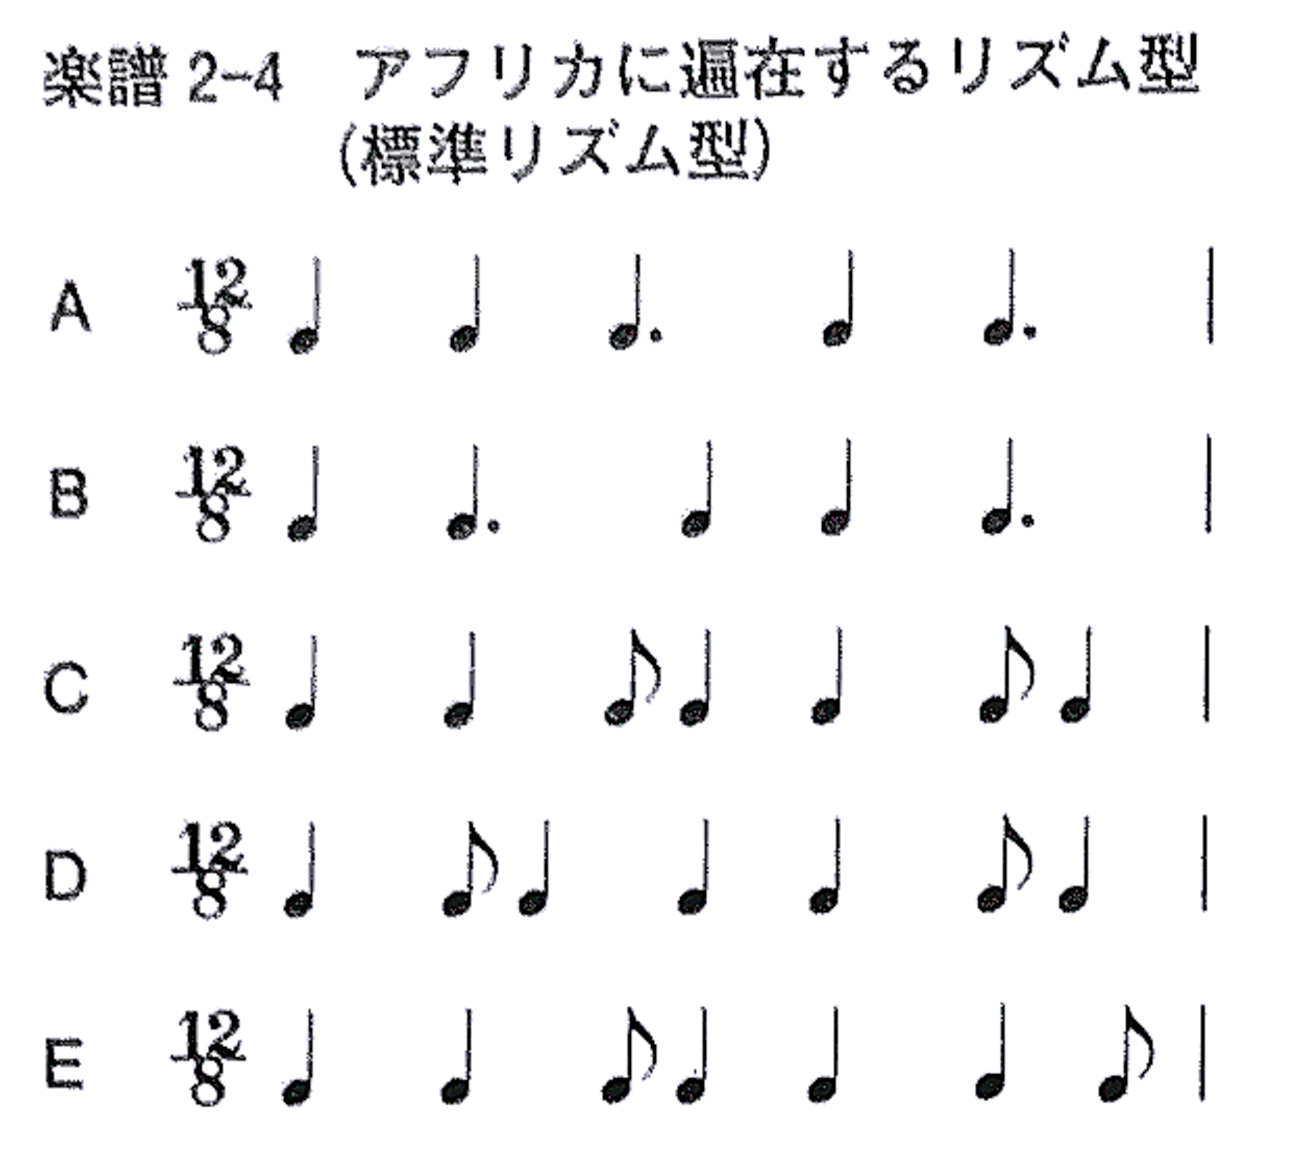
\includegraphics[
 width=0.5\textwidth]{./PDF/figure_15.pdf}
}
\caption{Kenichi Tsukada (\textit{The Truth About African Music} p.59, Score 2-4, 2016)}
\label{fig:figure_15}
\end{figure}

\begin{figure}[ht]
\centerline{
	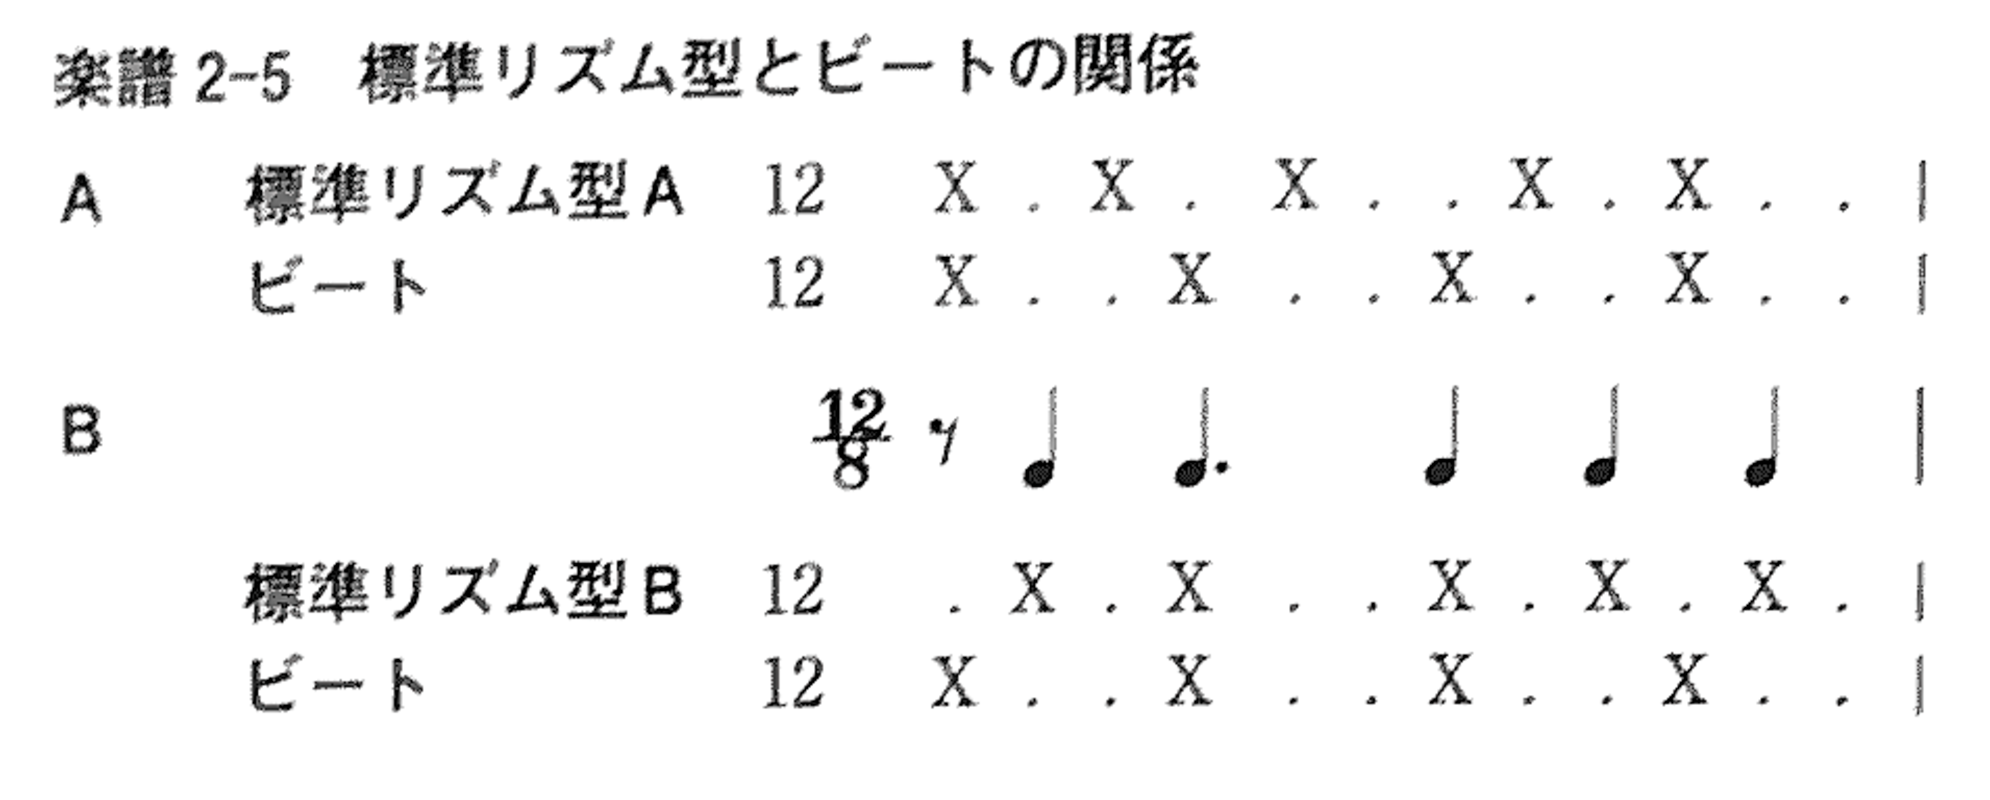
\includegraphics[
 width=0.75\textwidth]{./PDF/figure_16.pdf}
}
\caption{Kenichi Tsukada (\textit{The Truth About African Music} p.61, Score 2-5, 2016)}
\label{fig:figure_16}
\end{figure}

\subsubsection{Definition of Polyrhythm/Cross-rhythm}

As discussed above, the general interpretation of "polyrhythm" is broad, but when examining African polyrhythm, a certain structure can be identified. Regarding this structure, Kikuchi and Otani state: "\textbf{The cross-rhythm of 3 and 4 is, by my definition, no longer polyrhythm. That is African-style monorhythm (omitted). Only when you enter into the accents or the contraction of time sense that arises from it do you enter the African polyrhythmic stage (omitted). In today's commercial music, I would like to consider the 3 and 4 cross we just did as fundamental}"\cite{kikuchi-ootani:01}. Tsukada also points out, as an example of vertical hemiola appearing in commercial music, "\textbf{in the song 'Polyrhythm' (composed by Yasutaka Nakata) that the Japanese techno-pop unit Perfume hit in 2007, a powerful and impressive vertical hemiola structure appears in the interlude section}"\cite{tsukada:01}.

Therefore, "polyrhythm/cross-rhythm" in this thesis is defined as follows, based on Kikuchi and Otani's definition:

\begin{description}
 \item[Cross-rhythm]\mbox{}\\
	    Two or more time signatures that divide one cycle unit by integer ratios. Vertical hemiola-type rhythm.
 \item[Polyrhythm]\mbox{}\\
	    Two or more time signatures that do not divide one cycle unit by integer ratios. Rhythm with sway or accent.
\end{description}

According to this definition, the 12-beat cycle rhythm with 3-beat and 4-beat pulses, previously considered the basic African polyrhythm, has 12 as its least common multiple and is classified as cross-rhythm. A polyrhythmic state would be, in a simple example, a rhythm with 4-beat and 5-beat pulses against a 12-cycle: dividing 12 beats by 4 yields a beat unit of 3 beats, which divides evenly as an integer, but dividing by 5 results in a beat unit of 2.4 beats, which does not divide evenly.

Based on this definition, we will now examine the polyrhythmic/cross-rhythmic situations in India, the Middle East, and Latin music.

\subsubsection{India}

In Indian music, there exists a rhythmic form called tala, which "\textbf{takes the form of measures similar to Western music, but has created many types of time division arrangements}"\cite{deva:01}. Tala is "\textbf{defined as an arrangement with periodicity of a certain pattern}"\cite{deva:01}, and "\textbf{the essence of tala lies in its periodicity and repetitiveness}"\cite{deva:01}. Regarding the polyrhythmic/cross-rhythmic nature of Indian music using tala, Sachs indicates this in \textit{Rhythm and Tempo} with the terms "contrapuntal rhythm" and "overlap of two patterns."

First, regarding "contrapuntal rhythm," he states: "\textbf{Simple contrapuntal rhythm uses the same tala. That is, one hand plays the pattern at standard tempo, while the other hand expands its length}"\cite{sachs:01}. Figure \ref{fig:figure_17} illustrates this.

\begin{figure}[ht]
\centerline{
	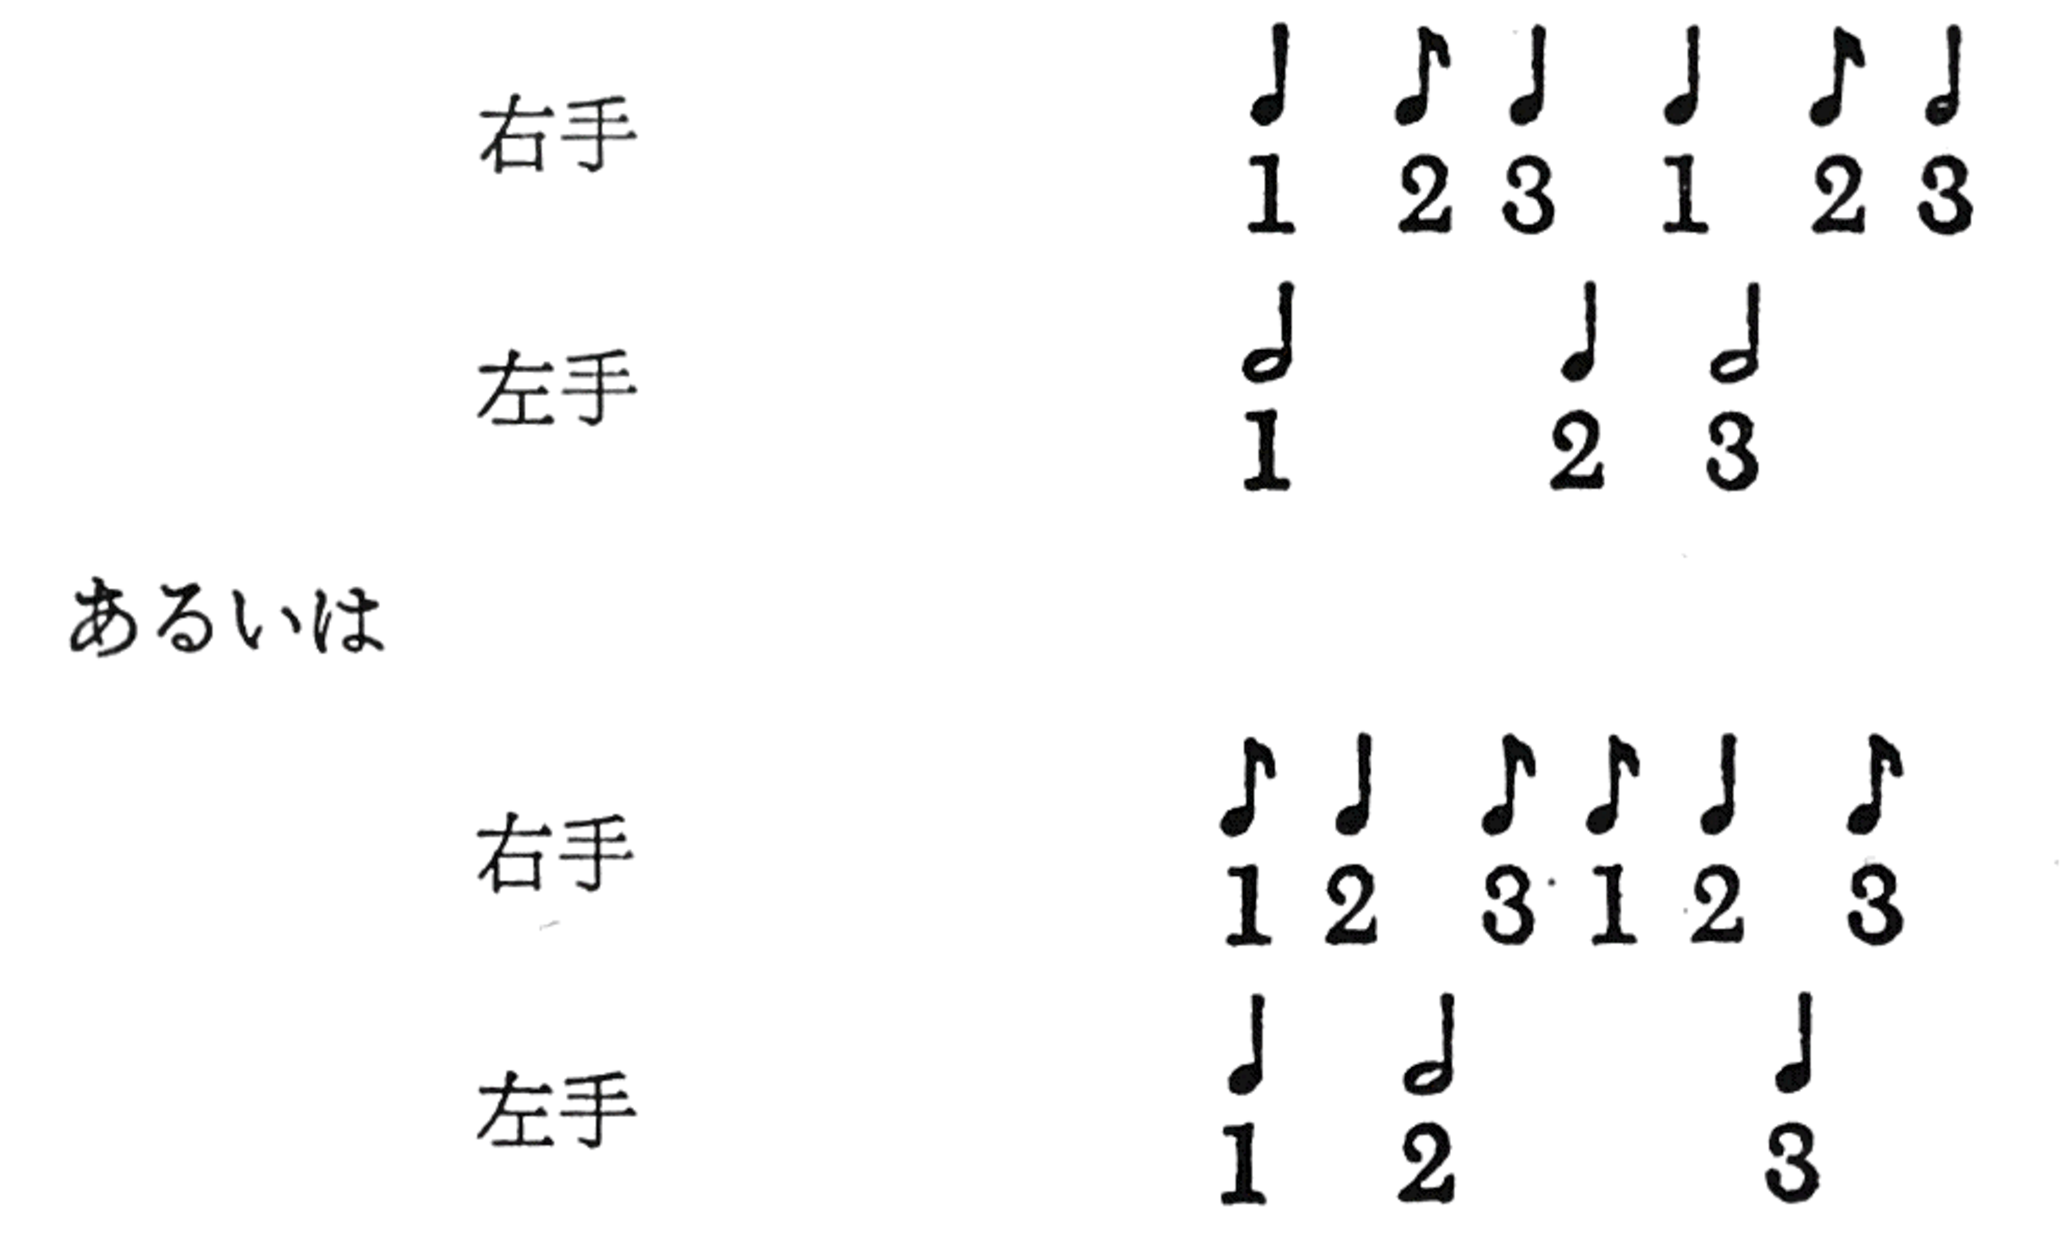
\includegraphics[
 width=0.5\textwidth]{./PDF/figure_17.pdf}
}
\caption{Curt Sachs (\textit{Rhythm and Tempo} p.106, 1979)\\
Example of oppositional rhythm. The left hand is expanded to twice the length of the right hand's rhythm.}
\label{fig:figure_17}
\end{figure}

As another example of "contrapuntal rhythm," he states: "\textbf{It frequently happens that both hands play different talas. As follows, one hand plays at standard tempo while the other hand plays at expanded tempo}"\cite{sachs:01}, showing this in Figure \ref{fig:figure_18}.

\begin{figure}[ht]
\centerline{
	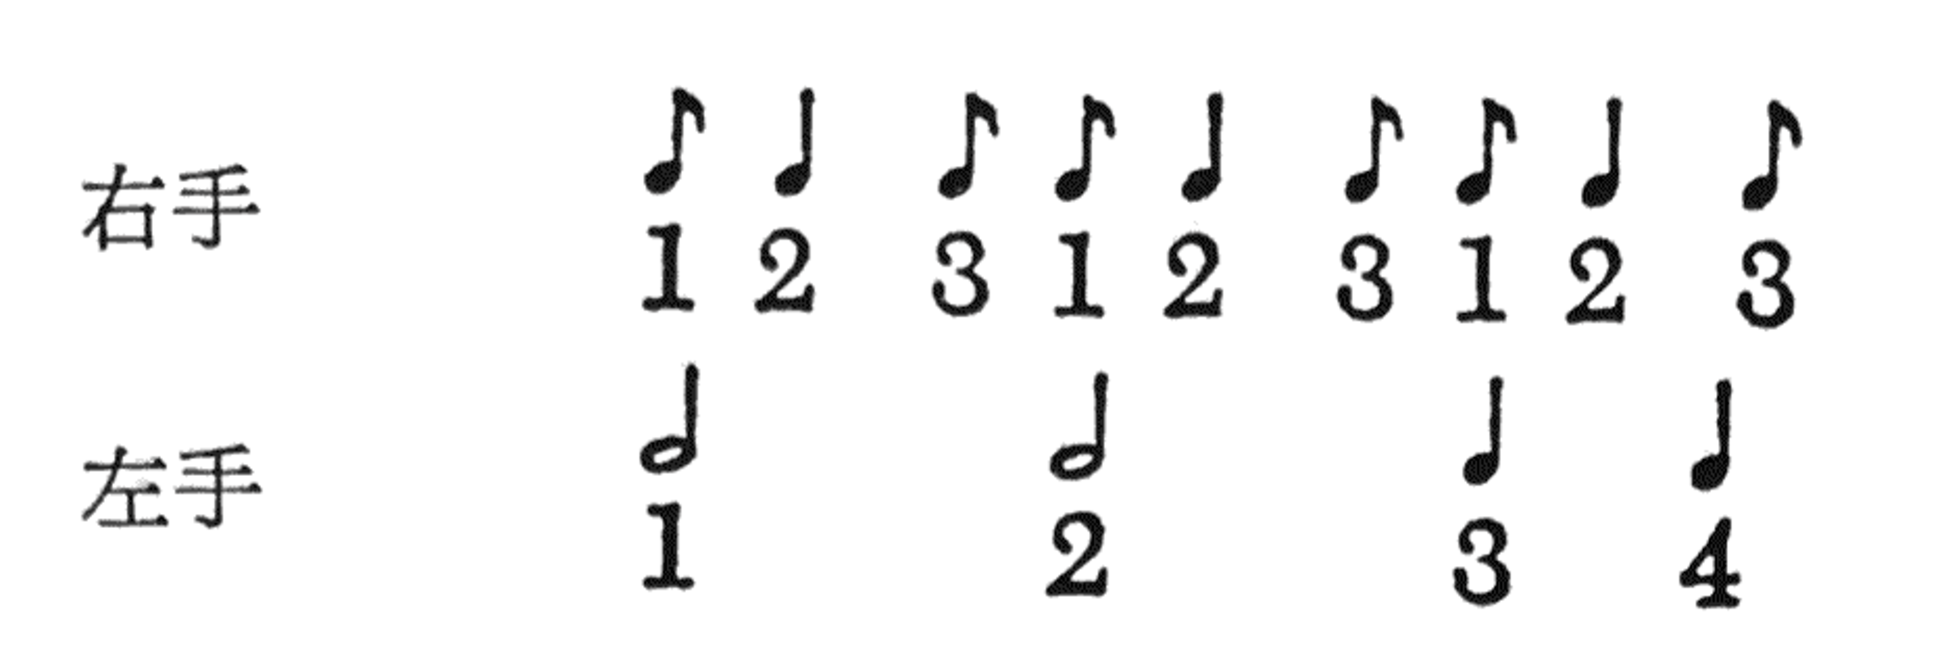
\includegraphics[
 width=0.5\textwidth]{./PDF/figure_18.pdf}
}
\caption{Curt Sachs (\textit{Rhythm and Tempo} p.107, 1979)\\
Example of performing different talas with right and left hands}
\label{fig:figure_18}
\end{figure}

As an example of "overlap of two patterns," he presents Figure \ref{fig:figure_19}.

\begin{figure}[ht]
\centerline{
	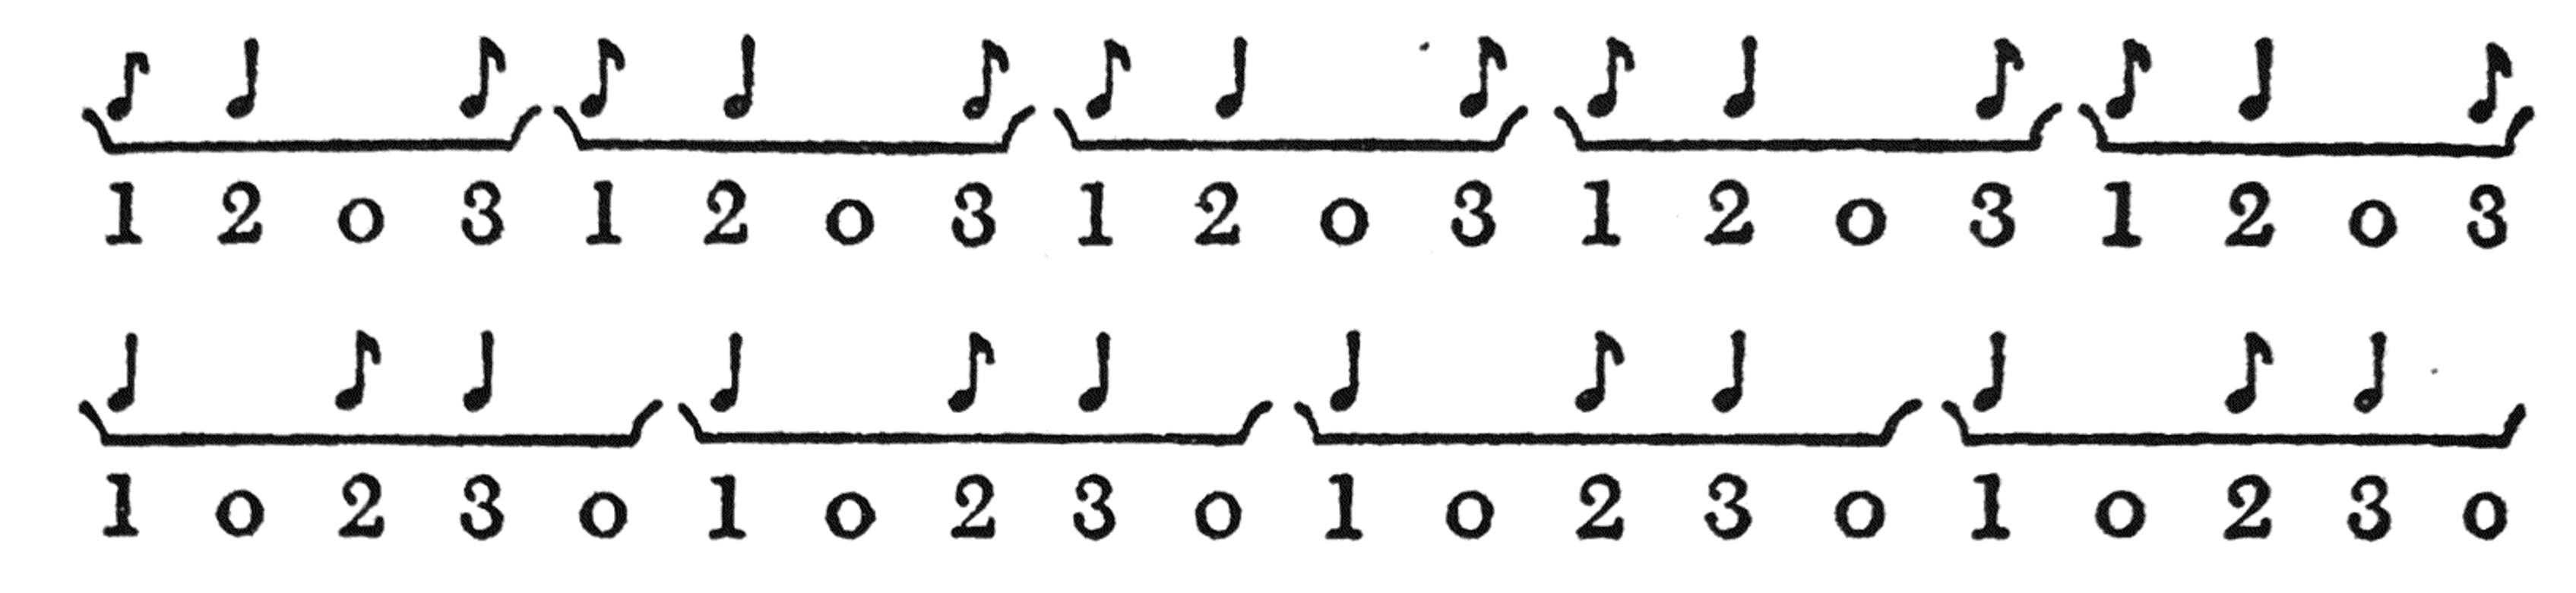
\includegraphics[
 width=0.7\textwidth]{./PDF/figure_19.pdf}
}
\caption{Curt Sachs (\textit{Rhythm and Tempo} p.108, 1979)\\
Example of overlap of two patterns. The same structure as African vertical hemiola can be observed.}
\label{fig:figure_19}
\end{figure}

According to our earlier definition of polyrhythm, this form is a cross-rhythm of 5-beat and 4-beat in a 20-beat cycle, and we can confirm similar rhythms in Indian music as well.

% %改ページや図版を章に収めたい場合は以下のように改ページすると収まる。
% \afterpage{\clearpage}
% \newpage

\subsubsection{Middle East}

According to \textit{Arab Music} by Salah al-Mahdi, Middle Eastern rhythms have rhythm patterns called iqa'. Mahdi describes Arab rhythms as "\textbf{a rhythm system peculiar to Arabic-speaking peoples}"\cite{mahdi:01} and "\textbf{originally linked to poetic meter (omitted), which gradually became somewhat independent}"\cite{mahdi:01}. Sachs also states that "\textbf{Arabian music originally followed the rhythm of poetry}"\cite{sachs:01}. Regarding the polyrhythmic nature of Middle Eastern music (Sachs refers to it as Near Eastern), Sachs states: "\textbf{When the three elements of sound—loudness, timbre, and beat—occur simultaneously, a complex aggregate of meter and accent is created within any single pattern that is almost polyrhythmic. It is infinitely variable in length, in the distribution of accent and timbre, and has varied}"\cite{sachs:01}. According to our earlier definition, while this is polyrhythmic in a broad sense, I was unable to find similar cases of the clear cross-rhythm forms seen in Indian music.

% 図\ref{fig:figure_20}にあるチェニジアの例を上げている。

% \begin{figure}[ht]
% \centerline{
% 	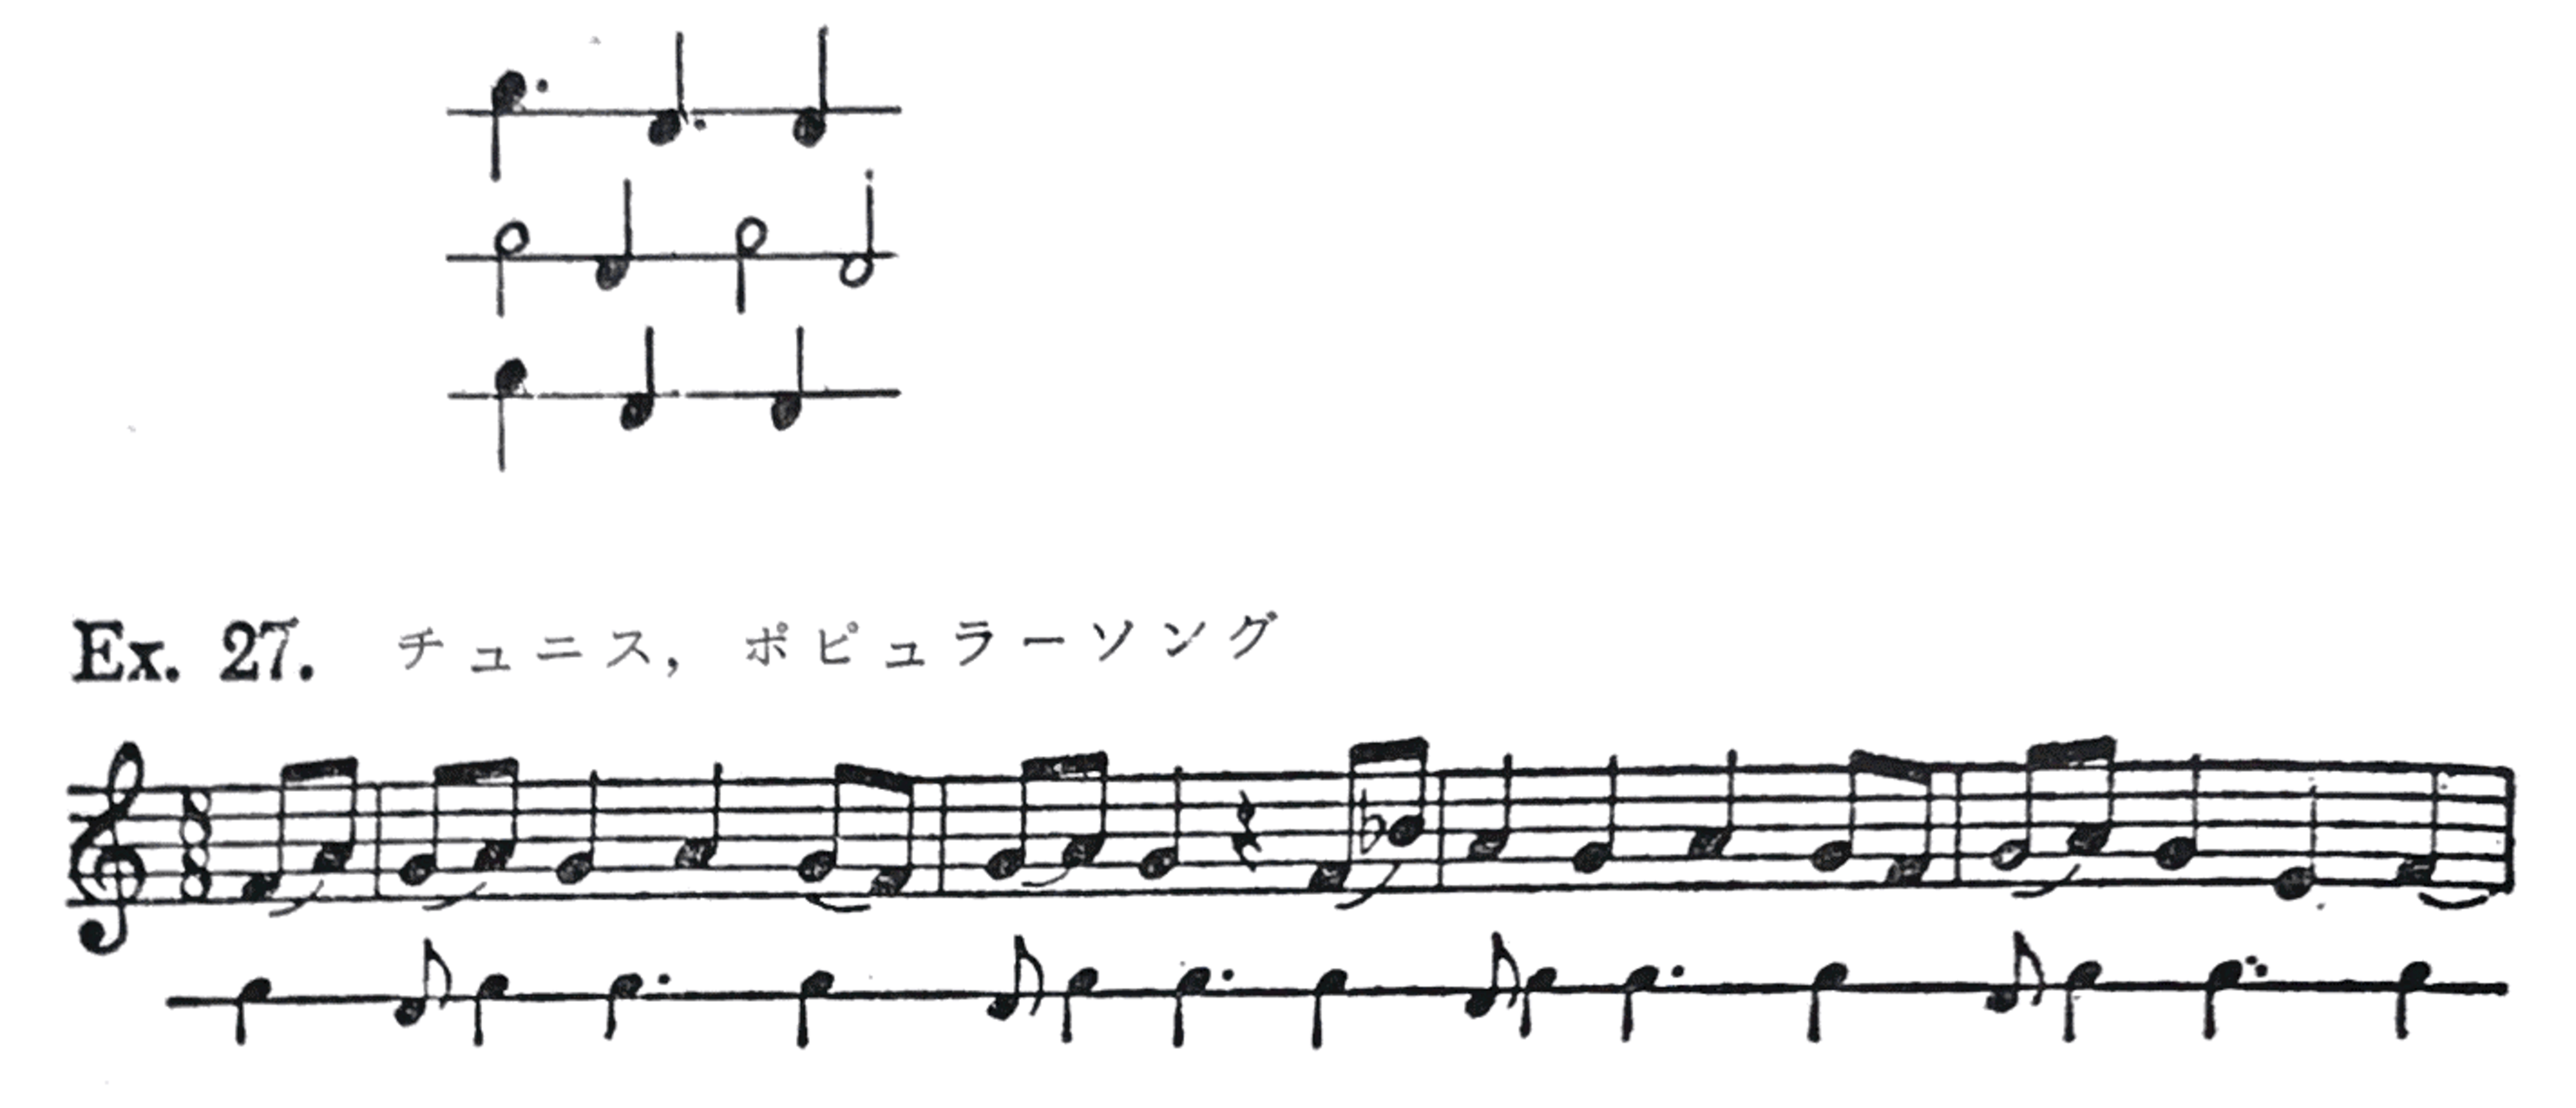
\includegraphics[
%  width=\textwidth]{./PDF/figure_20.pdf}
% }
% \caption{クルト・ザックス (『リズムとテンポ』p88, 1979)\\
% 譜例は上段の歌に対して下段のリズムが特に周り混むこともなくアフリカやインドの例のような明確なクロスリズムの形を持っていない}
% \label{fig:figure_20}
% \end{figure}

\subsubsection{Latin}

Regarding Latin rhythms, we will examine the clave, a rhythm pattern that is "\textbf{the cornerstone of Latin music}"\cite{yubi:01}, struck by claves, a percussion instrument from Central and South America. Tsukada states: "\textbf{What is interesting is that this standard rhythm pattern is thought to have formed the basis of the Latin music rhythms we often hear today}"\cite{tsukada:01}. He also points out the similarity: "\textbf{When examining the rhythms of Afro-Cuban music, for example rumba, in detail, there is a strong kinship between the clave and the standard rhythm pattern}"\cite{tsukada:01}. He also simultaneously points out that "\textbf{rumba preserves the characteristics of African rhythm structure extremely well, with 3-beat system (6/8 time or 12/8 time) rhythms and 2-beat system (2/4 time or 4/4 time) rhythms proceeding simultaneously in separate parts. In other words, it has a polyrhythmic structure}"\cite{tsukada:01}.

Figure \ref{fig:figure_21} shows this similarity and polyrhythmic structure. From this figure, it can be inferred that "\textbf{what occurs when trying to perform standard rhythm pattern A (author's note: referring to the standard rhythm pattern of 2-9 in the figure) not in the original 3-beat system but in a 2-beat system is the clave rhythm system}"\cite{tsukada:01}.

Furthermore, the rhythm called "tresillo" (Score 2-11 in Figure \ref{fig:figure_21}), derived from this clave, "\textbf{including its variations, has been extensively used not only in Latin music but also in rhythm and blues, jazz, rock and roll, and has had an enormous influence on the formation and development of popular music worldwide thereafter. And the rhythm that became the origin of this (omitted) was the standard rhythm pattern of traditional African music}"\cite{tsukada:01}. Thus, the African musical origins of popular music can be recognized "\textbf{not as subjective impressions or speculations with weak grounds, but as discourse consistent with historical facts derived from music analysis}"\cite{tsukada:01}. I believe this validates the methodology of approaching the development of popular music in this research from "polyrhythm/cross-rhythm" from a music historical perspective.

\begin{figure}[ht]
\centerline{
	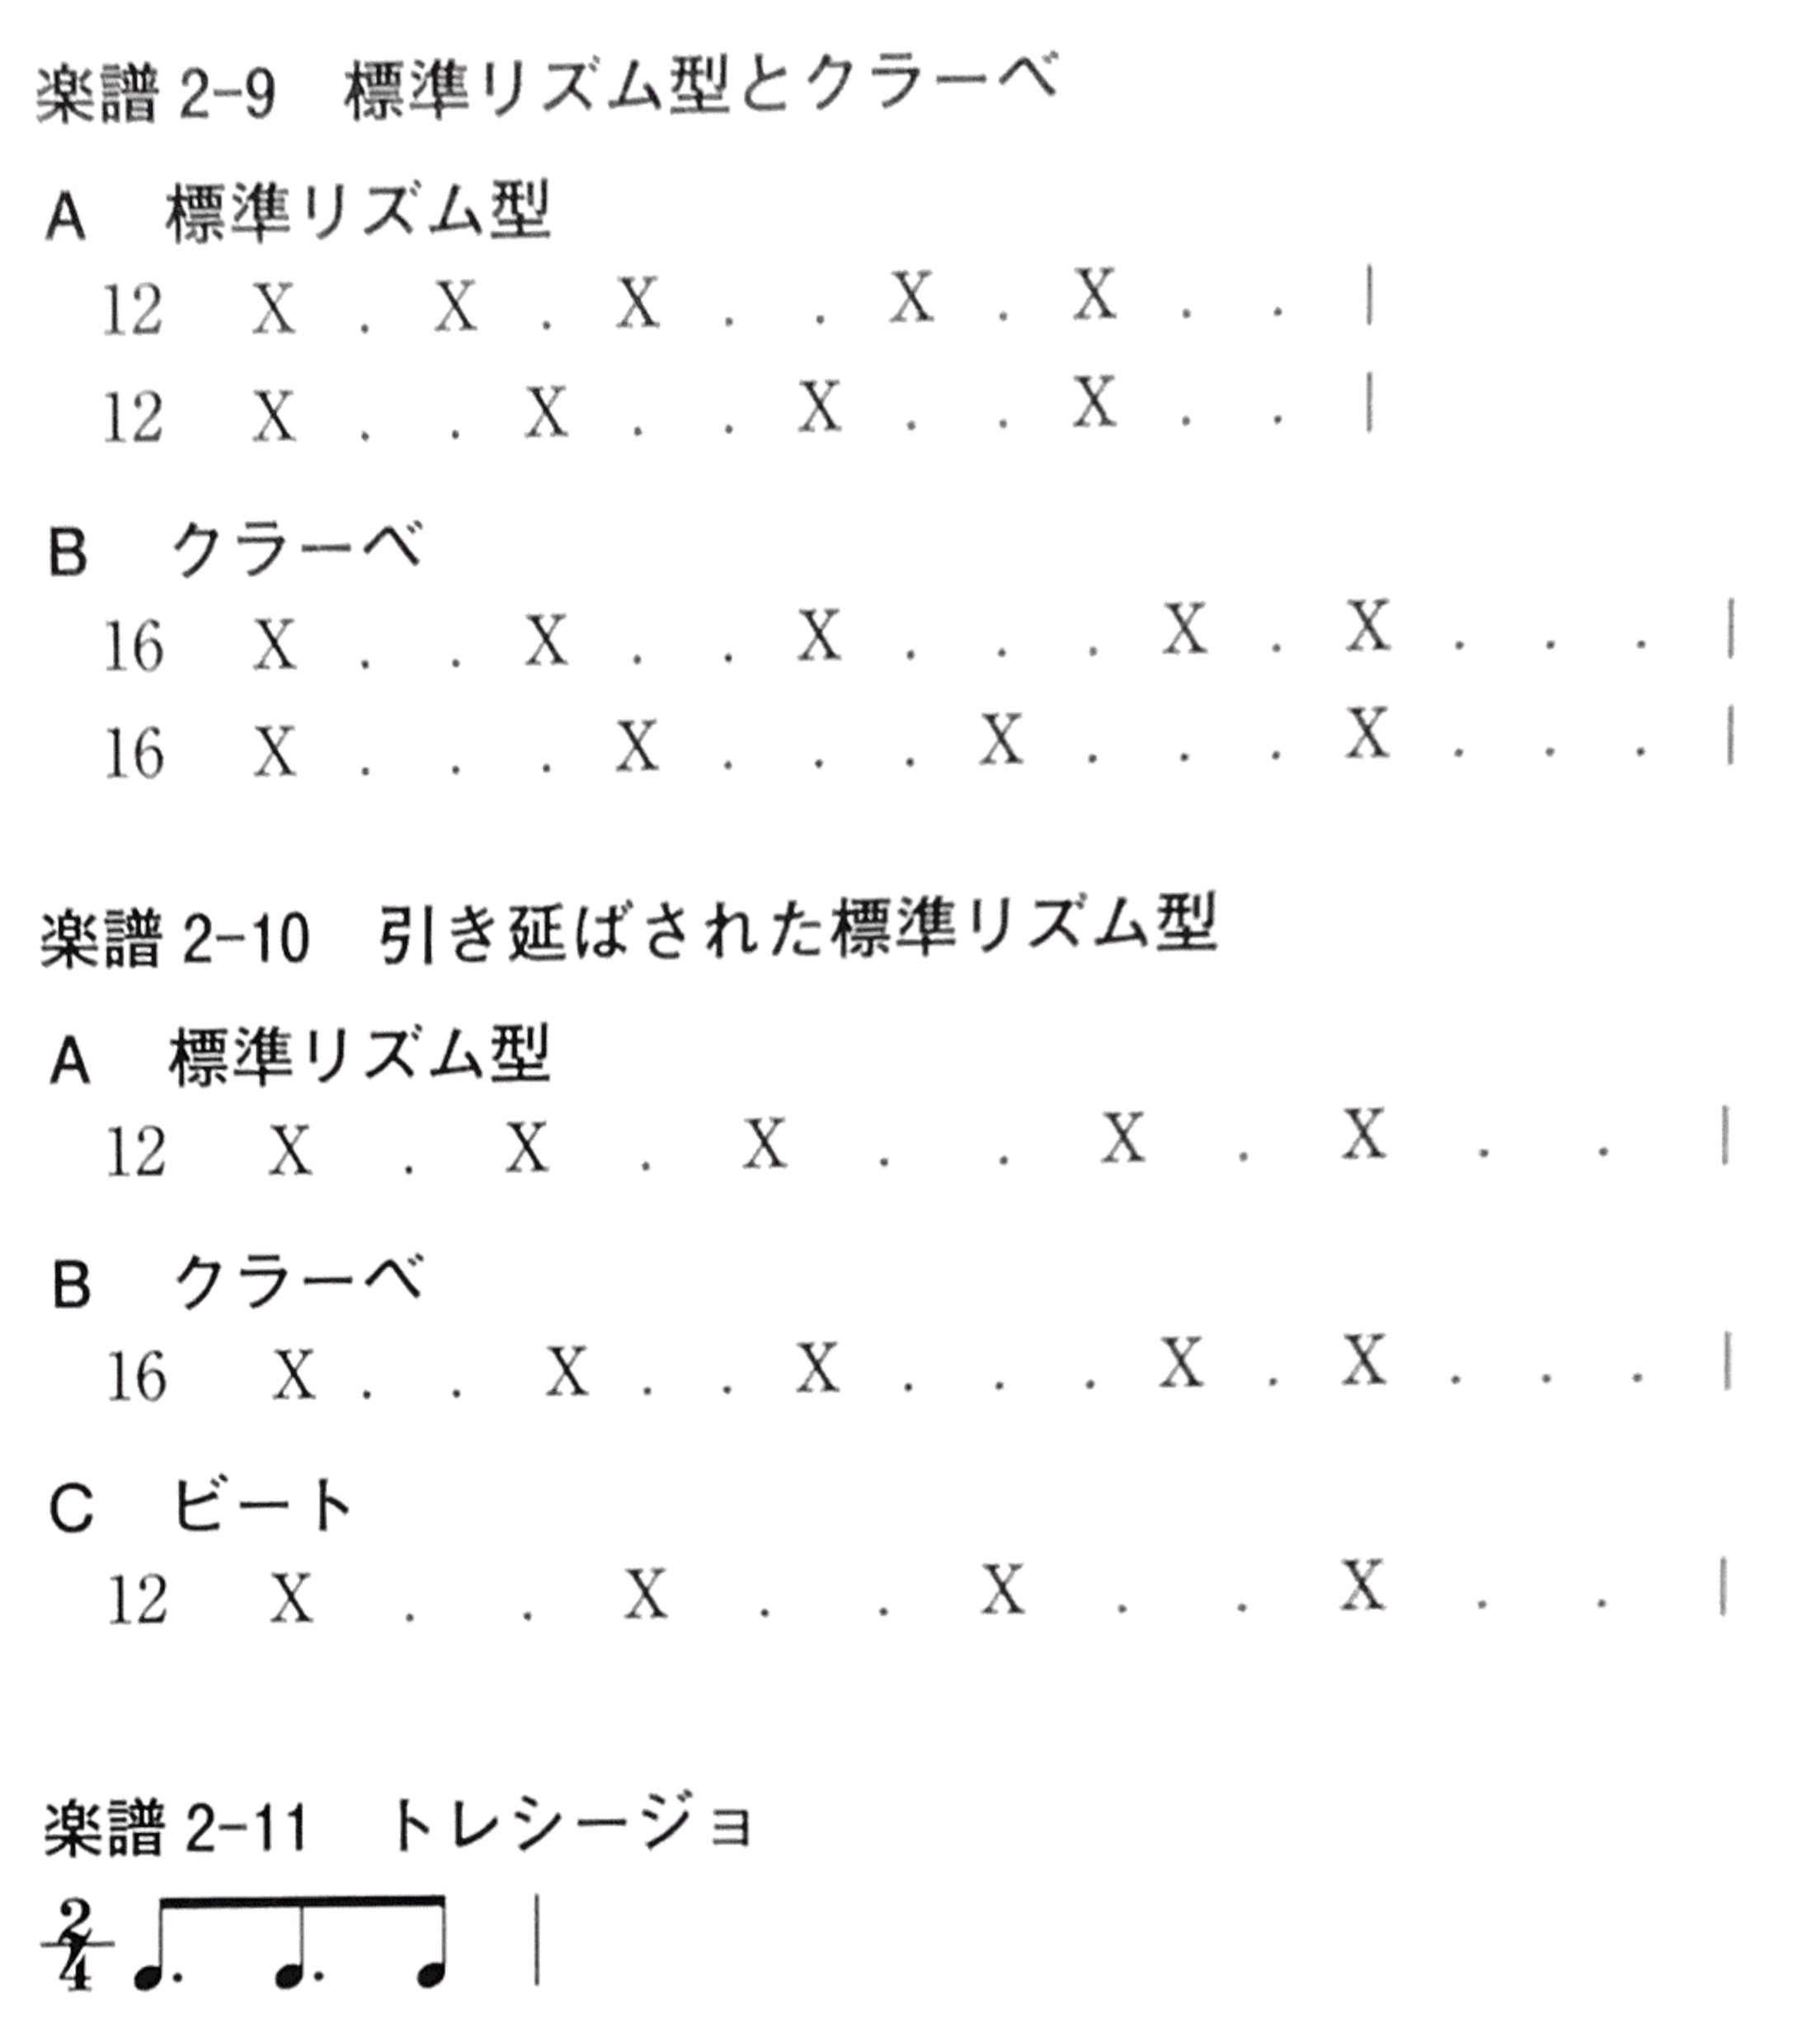
\includegraphics[
 width=0.75\textwidth]{./PDF/figure_21.pdf}
}
\caption{Kenichi Tsukada (\textit{The Truth About African Music} p.75 Scores 2-9, 2-10, 2-11, 2016)\\
Figures showing the similarity between African standard rhythm patterns and the clave, and tresillo patterns}
\label{fig:figure_21}
\end{figure}

Furthermore, the "polyrhythmic nature" of the clave and its relationship to "African basic rhythms" can be examined through rhythm strike points illustrated using waveforms in \textit{Rumba Clave: An Illustrated Analysis}. This analysis clearly shows the strike points of the clave in 4/4 time and 12/8 time, then compares the strike points of ten different performers. From this comparison, traces of Tsukada's "African origins of the clave" can be observed. Additionally, the fluctuation of strike points between 4/4 time and 12/8 time can be visually observed, and although it does not superficially take the form of cross-rhythm, the fact that the clave is of African origin and that such rhythm with "sway" and "accent" is one manifestation of the "African polyrhythmic stage" as cited in Kikuchi and Otani's definition of polyrhythm earlier. If "\textbf{Spanish-Cuban people who had not acquired the African-specific way of feeling the basic pulse of the standard rhythm pattern heard the standard rhythm pattern as a rhythm pattern consisting of 16 pulses}"\cite{tsukada:01}, then even according to our earlier definition, this can be said to be extremely polyrhythmic music.

\subsection{Polyrhythm/Cross-rhythm in Western Music}
\subsubsection{Western Music, Contemporary Music, American New Music \label{Western-Modern-AmericanNewMusic}}

Regarding "polyrhythm/cross-rhythm" in Western music, the \textit{New Music Dictionary} (40th edition, 1996) again states: "\textbf{Examples of polyrhythm (metric) are found mostly in the 14th-15th centuries and the 20th century, and this phenomenon is closely related to music being free from tonal function and functional harmony}"\cite{asaka:01}. Figure \ref{fig:figure_22} is the musical example illustrated there.

\begin{figure}[ht]
\centerline{
	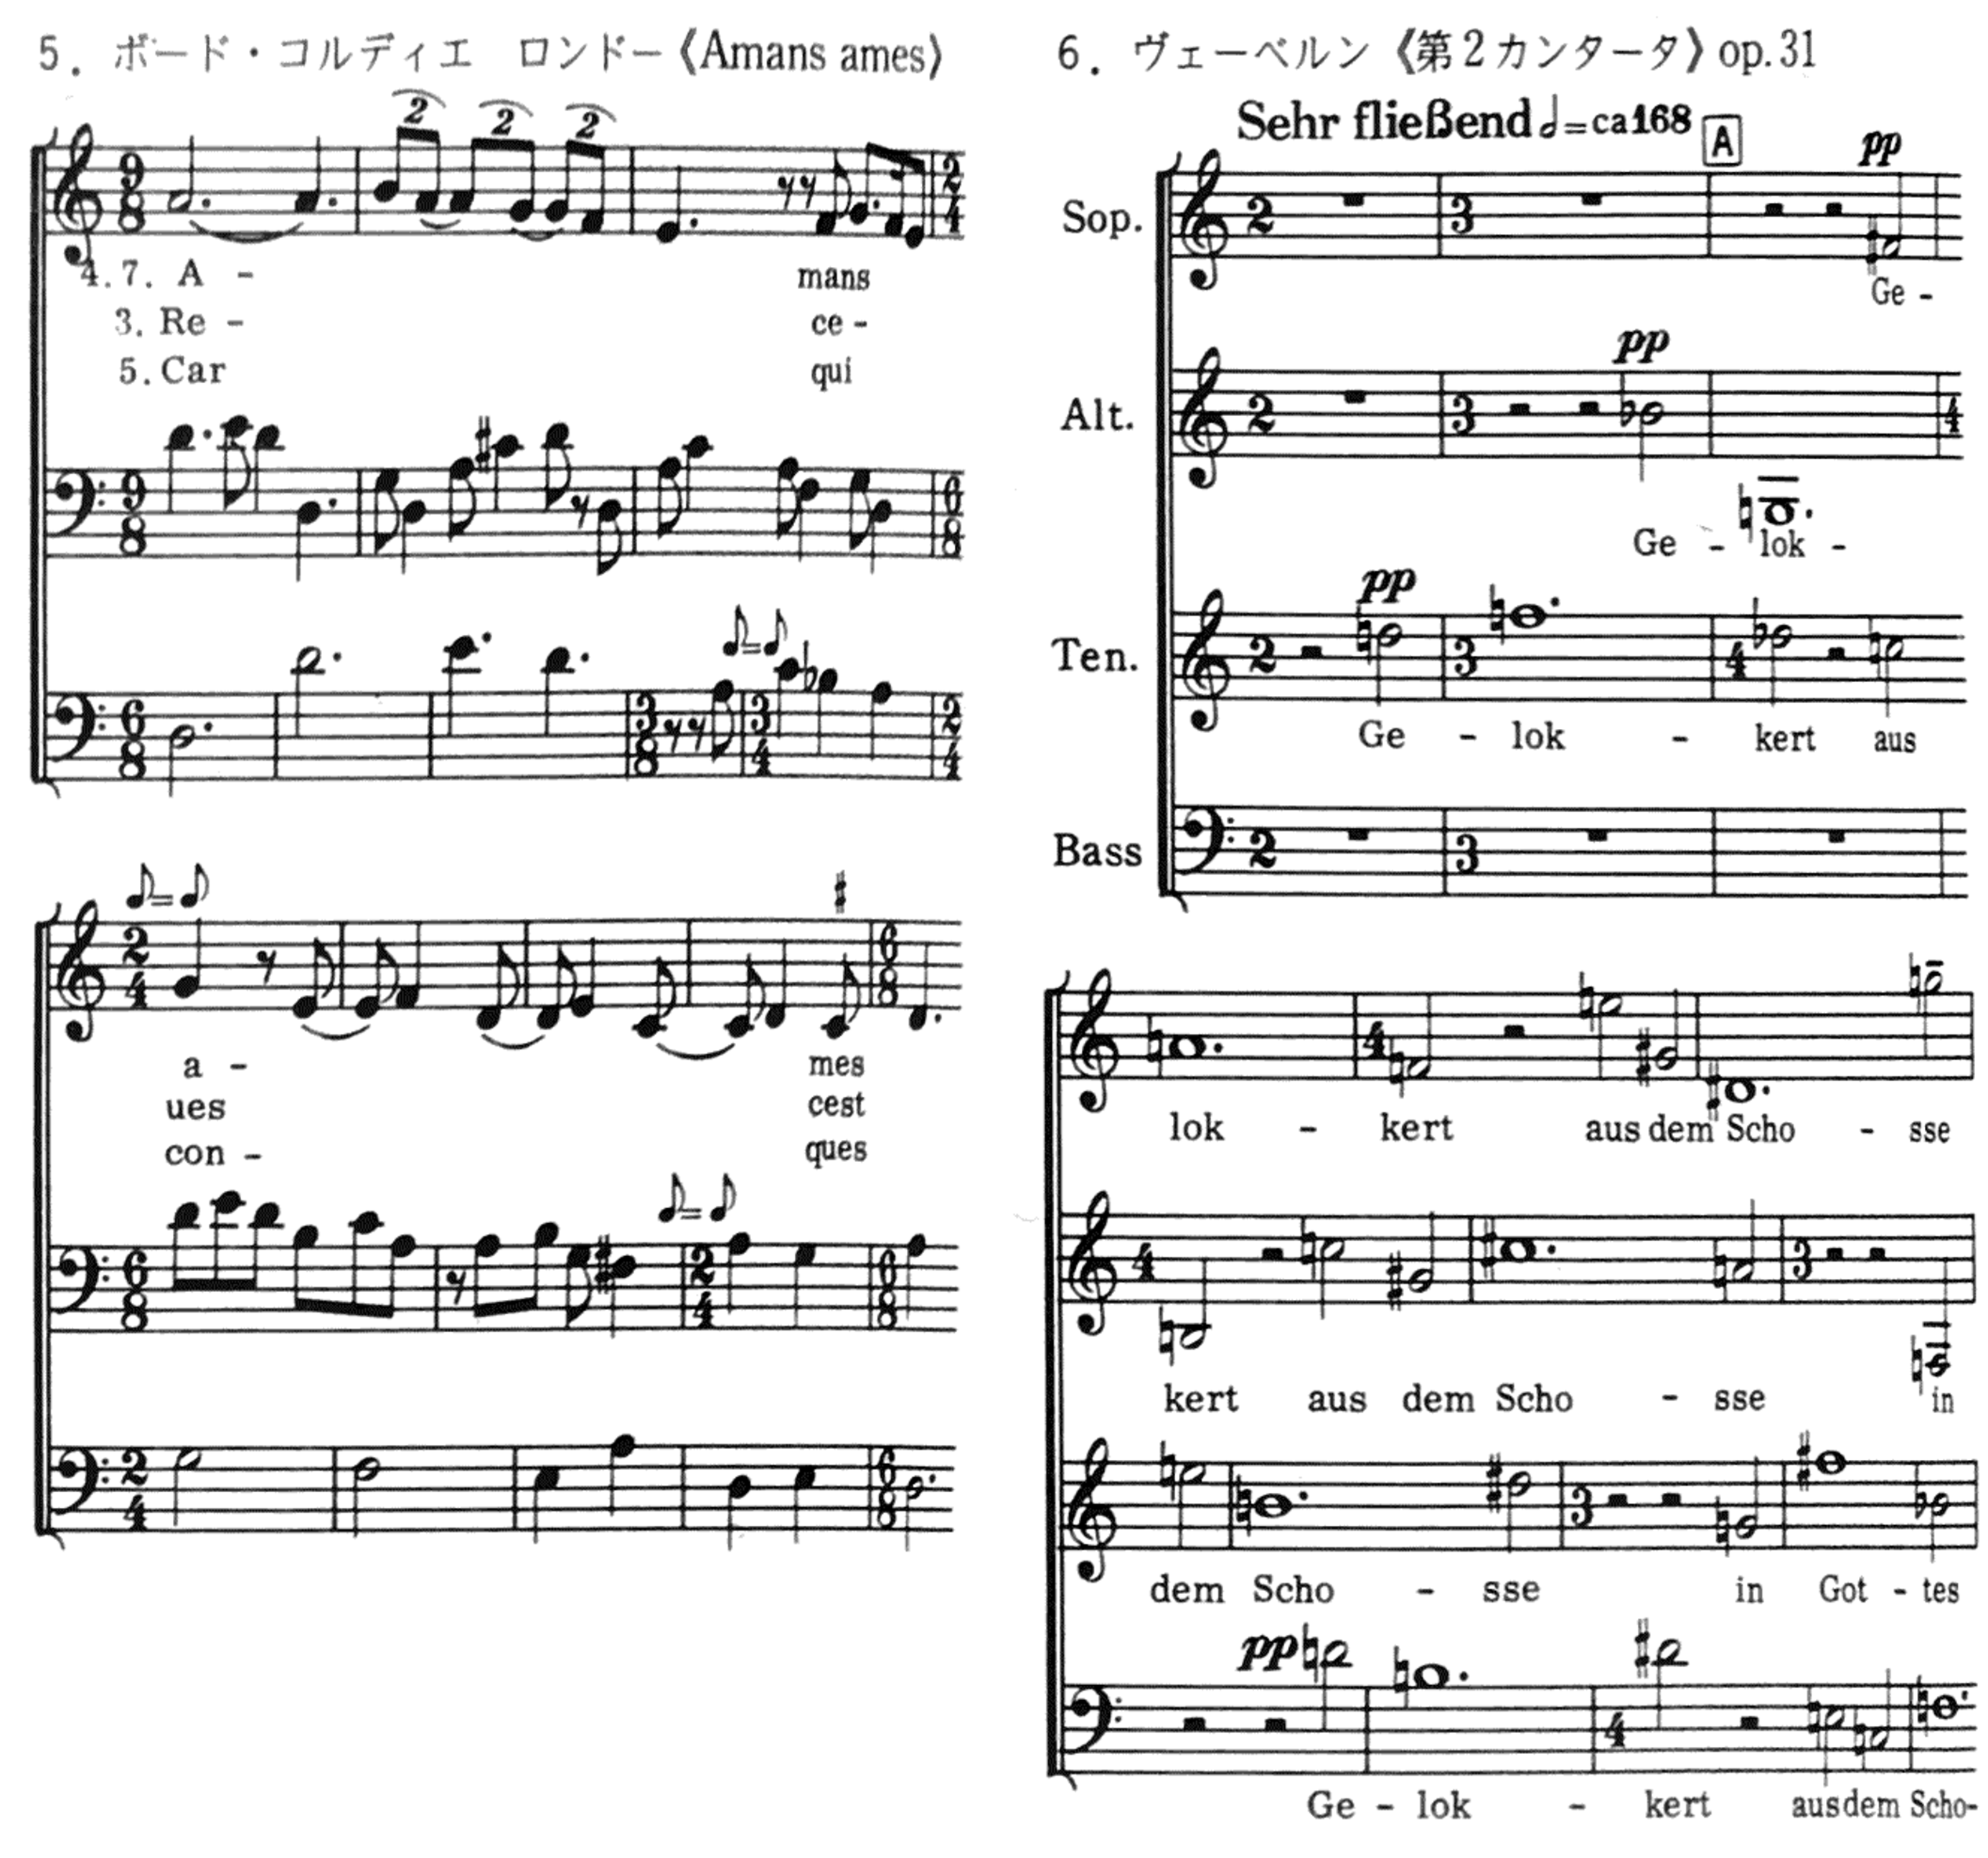
\includegraphics[
 width=0.75\textwidth]{./PDF/figure_22.pdf}
}
\caption{Jun Asaka (\textit{New Music Dictionary} p.538, Examples 5 and 6, 1977)\\
Example where bar lines wrap around due to different time signatures in different staves}
\label{fig:figure_22}
\end{figure}

Regarding the period before Baroque, Sachs's \textit{Rhythm and Tempo} also addresses polyrhythm up to the Renaissance with "alternation of meter" and "flamboyant polyrhythm," citing examples from late Renaissance composer Cipriano de Rore's "Vergine pura" (Figure \ref{fig:figure_23}).

\begin{figure}[ht]
\centerline{
	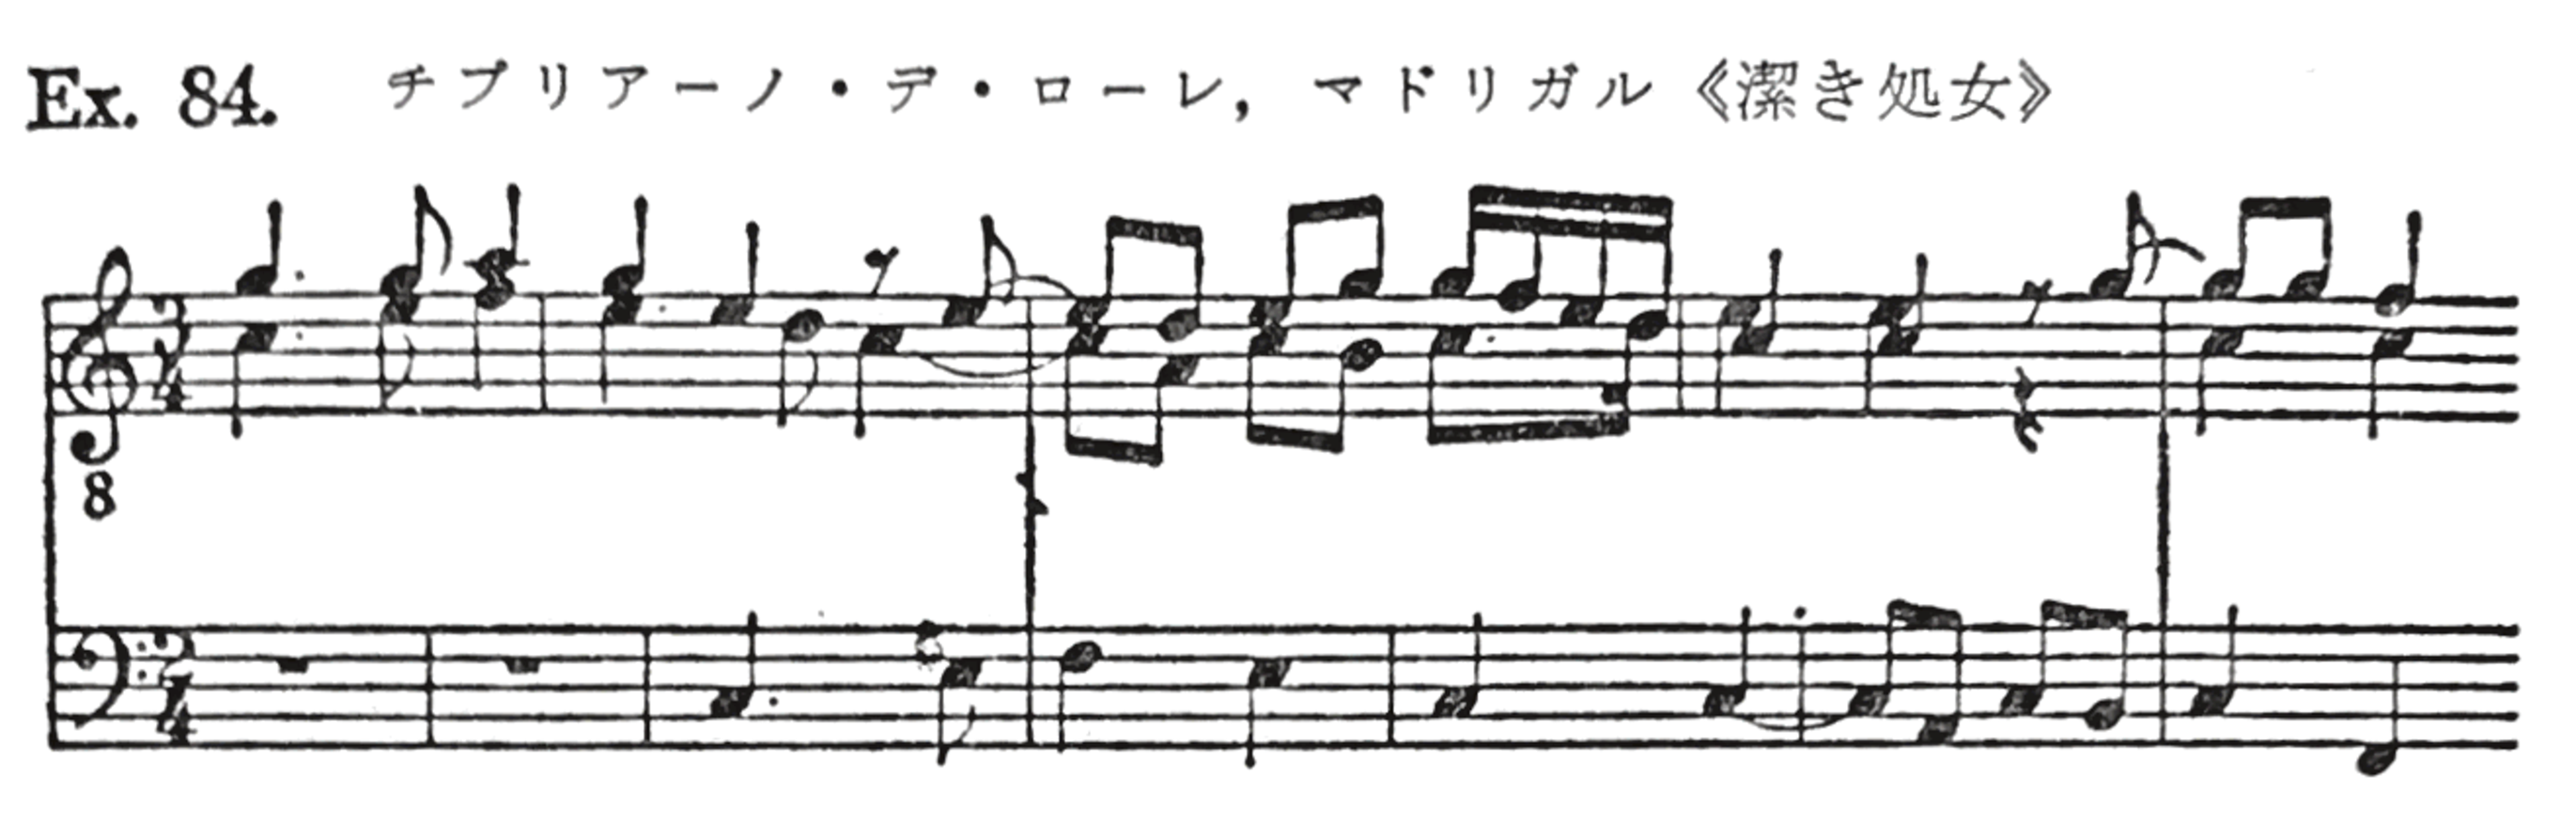
\includegraphics[
 width=0.75\textwidth]{./PDF/figure_23.pdf}
}
\caption{Curt Sachs (\textit{Rhythm and Tempo} p.272 Ex. 84, Cipriano de Rore's "Vergine pura" example, 1979)\\
Like Figure \ref{fig:figure_22}, bar lines wrap around due to different time signatures in different staves, but no form like cyclical rhythm patterns is observed}
\label{fig:figure_23}
\end{figure}

Entering the Baroque period, "polyrhythmic/cross-rhythmic" rhythms can be observed in hemiola structures in relation to dance, but cannot be seen as characteristic of musical rhythm. Furthermore, although 4/4 time established its leading position during the Baroque period, this also became the foundation for rhythms in subsequent Western music and popular music. Reich points out: "\textbf{What can be said about Baroque music in general, but especially Bach, is that the beat is constant and basically there is no ritardando or accelerando (omitted). What should be done is to maintain tempo}"\cite{strickland:01}, from which it can be understood that Baroque period rhythms had ceased to possess polyrhythmic elements.

Entering the 20th century, Reich can be recalled as one of the contemporary music composers who approached "polyrhythmic/cross-rhythmic" rhythms. While phase shifting is Reich's representative technique taken up here, Reich speaks in interviews about how phase shifting is a variation of canon form, inspired by tape loop works ("\textbf{Oh my God! This relationship is amazing. But what is really interesting is the process of starting in unison and slowly going out of phase, which is actually a variation of the old Western music canon!}"\cite{obrist:01}). In the same interview, Reich states: "\textbf{When I performed with Arthur Murphy, who became a founding member of my first ensemble, we discovered that we could play without using tape. This was in 1967, and this became a major breakthrough, leading to 'Piano Phase,' 'Violin Phase' (1967), and subsequently 'Drumming' (1970-1971)}"\cite{obrist:01}, describing his series of phase shift works as canons characterized by temporal change that "shifts" rather than the "sway" or "accent" of African polyrhythm. However, when asked in another interview about the relationship with his experience learning Gamelan music, Reich states: "\textbf{(author's note: regarding Music for Mallet Instruments, Voices and Organ) I certainly listened to various recordings. Another example is 'Drumming.' I didn't write it because I went to Ghana. (omitted) The African element in that work—the repetitive pattern in 12/8 time—was already done in 'Piano Phase' and 'Violin Phase' in 1967. I went to Africa to confirm}"\cite{strickland:01}, using the basic African rhythm structure of 12/8 time repetition while denying that this was influenced by African music itself, stating it was influenced by earlier works. Therefore, I consider it difficult to position Reich's works within the earlier definition of "polyrhythm/cross-rhythm" from the composer's own views (interviews).

\subsection{Polyrhythm/Cross-rhythm in Popular Music}

Thus far, we have examined, albeit in a limited manner, rhythms practiced in Africa, India, the Middle East, Latin America, and Western music. To comprehensively discuss music, it could be said to be impossible unless one examines all examples of that music. Furthermore, regarding popular music, since it is music that is currently in progress, even if we limit its origins to American folk music such as jazz and blues, the difficulty of discussing it comprehensively increases dramatically. Therefore, we will introduce the activities of Kikuchi, one of the authors whose writings form the basis for this thesis's polyrhythm definition, between Kikuchi and Otani.

When examining Naruyoshi Kikuchi's activities, it becomes clear that he has performed numerous practical works and performances through polyrhythmic approaches. Here, we will take up \textit{Date Course Pentagon Royal Garden} (now dCprG) as one example. In \textit{The School That Taught Sensuality and Melancholy}, Kikuchi states about his musical piece \textit{PLAYMATE AT HANOI}\cite{works-kikuchi:01}: "\textbf{It's a cross of 4 and 3. (omitted) Integer polyrhythm}"\cite{kikuchi-ootani:01}. He does say that as the piece progresses, "4 and 3 become mixed," but this part of his statement indicates that this piece is first in a state of vertical hemiola, and according to this thesis's definition, in a state of "cross-rhythm."

Then, regarding the rhythm structure of \textit{structure I la structure de la magie monderne / Structure 1 (Structure of Modern Magic)}\cite{works-kikuchi:02} by the same band, he explains as follows in comparison to the earlier \textit{PLAYMATE AT HANOI}: "\textbf{The structure here is 4/4 and 5/4. That is, the feature is that 4-beat and 5-beat coexist, (omitted) not the divisible cosmos polyrhythm of 12 prime numbers like the previous work 'Playmate at Hanoi,' but a rhythm that sounds square from one perspective (taking it in 5-beat, it sounds like house music based on sixteenth notes), but sounds 'accented' from the other perspective (taking it in 4-beat, a stumbling tribal rhythm like Tsugaru folk song or African folk song can be heard). The brass riff is also made entirely of variations of only sixteenth notes, but because strike points are frequently placed at unusual strike points, there is an intention to mix the instability and pleasure of the step. Furthermore, the long melody of the synthesizer that appears first as magic is composed of triplets, and in terms of integer approximation, triplets are positioned between 4-beat and 5-beat, working like an adhesive between the two rhythms.}"\cite{kikuchi:01}. This explanation corresponds to an example that matches this paper's definition of "polyrhythm" based on Kikuchi and Otani's definition.

Even without such clear examples, the connection from African basic rhythms to Latin clave discussed earlier in the section on Latin music, and the fact that this has widely influenced popular music, also demonstrates that popular music constantly receives African polyrhythmic sensibility. Furthermore, looking at jazz, which was popular music of the early 20th century, comparing Western music and jazz, "\textbf{whereas in classical music all parts are dominated by harmony and interlock vertically with each other, in jazz, while dominated by harmony, the rhythm of each part is linearly or horizontally independent, often forming polyrhythm}"\cite{yubi:01}, which also suggests the influence of African polyrhythmic sensibility. Yubi also points out that "\textbf{the bebop movement beginning in the 1940s aimed to expand the degree of expression in improvisation, and by introducing accent shifts of small note values, formed a more powerful polyrhythm than swing feel}"\cite{yubi:01}. As an example of post-bebop jazz musicians' African polyrhythmic sense, Figure \ref{fig:figure_24} shows part of John Coltrane's solo in \textit{Bye Bye Blackbird}\cite{miles:03}. Here, Coltrane uses phrases in triplets over two beats on a 4/4 rhythm, expressing 6-beat time over 4-beat time.

\begin{figure}[ht]
\centerline{
	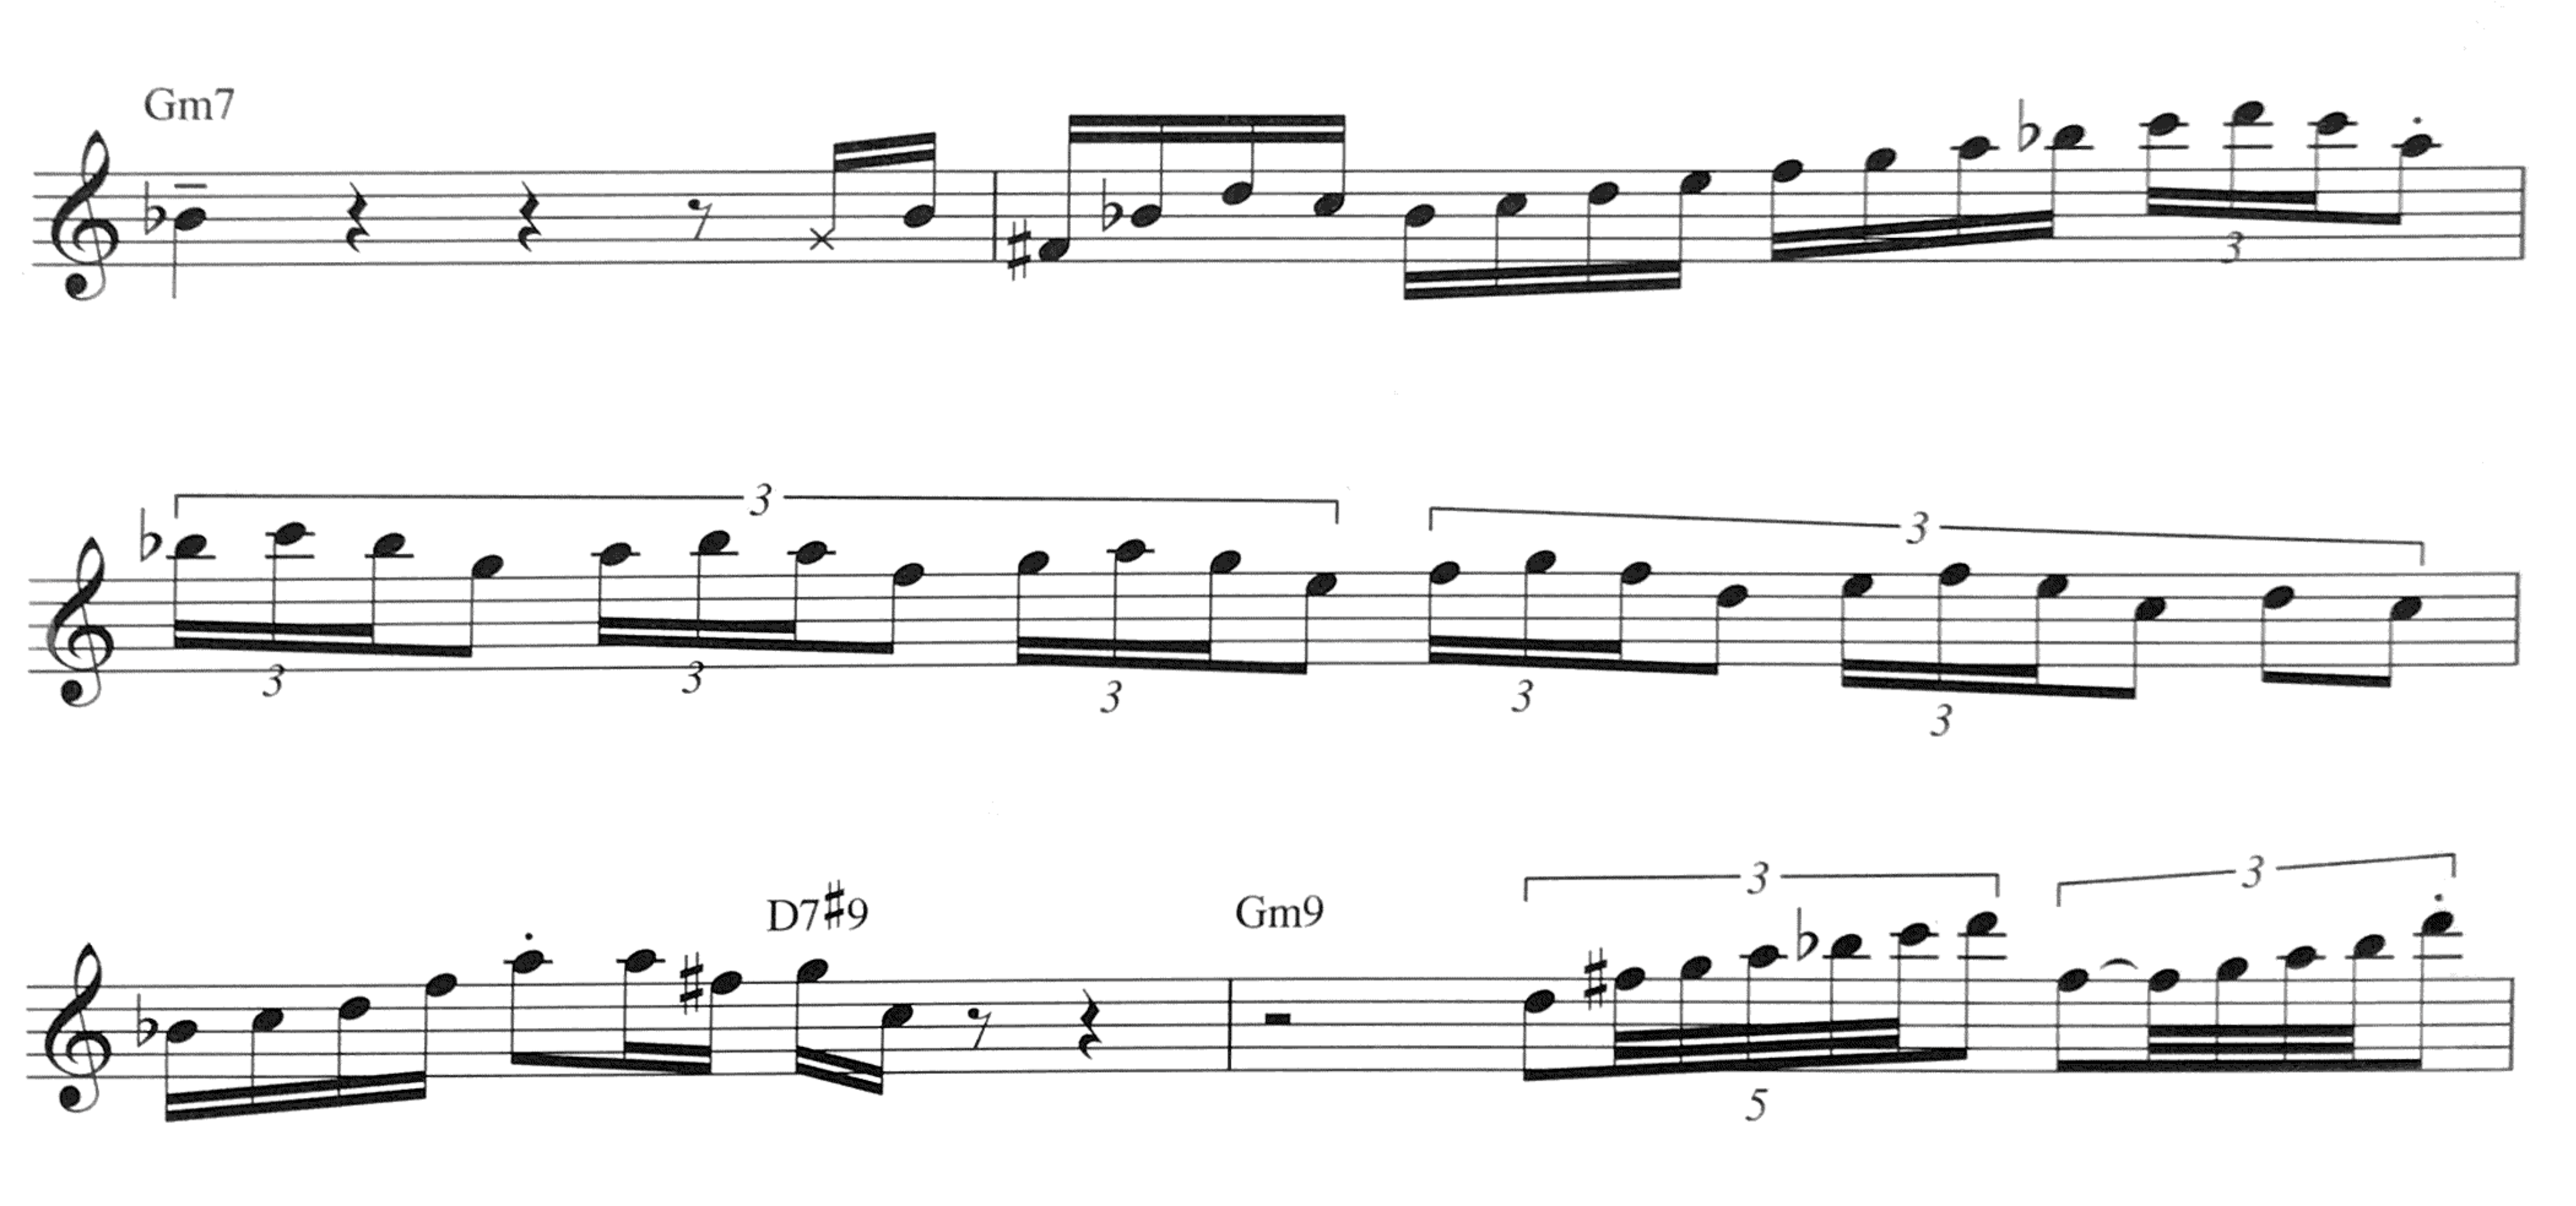
\includegraphics[
 width=\textwidth]{./PDF/figure_24.pdf}
}
\caption{Hal Leonard Corp (\textit{John Coltrane Omnibook: For C Instruments} p.50, excerpt from solo transcription of \textit{Bye Bye Blackbird}, 2013)\\
In the second measure of Example 3, entering with a 4-beat phrase in sixteenth notes, and using the phrase shape from the fourth beat of the same second measure as a motif, it becomes triplets over two beats in the third measure, dividing 4 beats into 6}
\label{fig:figure_24}
\end{figure}

Examples like Kikuchi's, where such division is applied throughout the entire piece, are not commonly found. However, entering the 21st century, the rhythmic "sway" and "accent" pointed out by Kikuchi and Otani have become increasingly observed, beginning with Robert Glasper's \textit{Black Radio}\cite{Glasper:02} released in 2012, and this can be said to be evidence of Kikuchi and Otani's definition as a contemporary manifestation of the African rhythmic sense that underlies popular music.

% ビジェイアイアー
%
% クラクラ
%
% これら総じて「揺れ」「訛り」をもった「ポリリズム的なリズム感覚」といっていいだろう。

% \subsection{考察}
%
% ーーーー執筆内容ーーーー\\
% 「ポリリズムやクロスリズムに関して人類はすでにこのようなことをやってきた。そして、それは事実、身体化可能なものだった」ということを説明したい\\
% クラシックの小節線ずれこみなども、基本的に周りこむ場合には拍が共有される場合が多く、アフリカンポリなどの訛りがあるポリの常態では小節線が共有される場合が共通して見られることを指摘する。そこに現代的なグルーブ感やリズム認知があると考えることが出来る。そこにはクラーゲスが言う「拍子(タクト)が同一のものを反復するとすれば、リズムでは類似が回帰する」ということに対するリズム回帰する力がポピュラー音楽に於いて強く働いていると仮説をたてる。\\
% ーーーー執筆内容ーーーー\\
%
% ここまでポリリズム/クロスリズムというリズムについてのアプローチを見てきた。
%
% またこの事は、五線譜による記譜法が17世紀以降に確立され、同時期に平均律による調性と和声に重きが置かれるようになったバロック時期には見られなくなったことを

% \section{現代の音楽制作環境と考察}
%
% 次に、先のポリリズム/クロスリズムの状況を現代の音楽制作環境から考察していく。考察にあたってはポピュラー音楽に於ける楽理、楽譜、制作環境としてのソフトウェアを取り上げる。
%
% \subsection{楽理的考察}
%
% ーーーー執筆内容ーーーー\\
% ハーモニックリズム、ドミナント進行、コードの共有、が一定のリズムフィギュア、もしくは小節という単位、にのってる点をバークリー理論や作曲法を引き合いに出して述べる。このあたりはザックスの本から拾えないか??\\
% ーーーー執筆内容ーーーー\\
%
% バロックでのリズムと和声の密接と4分の4拍子の支配的
%
% バークリー理論でのポピュラー音楽への展開
%
%
%
% \subsection{楽譜的考察}
%
% ーーーー執筆内容ーーーー\\
% で、上記の話を記述する楽譜自体が「拍と小節線の共有」という、所謂「行進」のような話とそういう音楽を記述する上で発展してきた背景が、システムとして全体を縛っている、という話を進める。ここは先の4/4が支配的になった話をして譜面のシステムとしての完成と自由度のバーターを論じる。\\
% ーーーー執筆内容ーーーー\\
%
% \subsection{ソフトウェア的考察}
%
% ーーーー執筆内容ーーーー\\
% その楽譜の考えかたで現代のソフトウェアは出来ているので、多様性が生じ難い土壌になっている。その上でそういう音楽がマスで流通するのだから、より4/4の支配力が増してるだろう事を指摘する。\\
% ーーーー執筆内容ーーーー\\

%改ページや図版を章に収めたい場合は以下のように改ページすると収まる。
\afterpage{\clearpage}
\newpage
